\section{Introduction}
\label{industry_needs}
As we mentioned in chapter \ref{chapter_general_intro}, despite the main aim of this thesis has been to derive a methodology for approximating the motivational state of individuals while interacting with potentially rewarding object (a videogame in this case), a secondary objective was to illustrate the potential application of this methodology within an industrial setting.

In this view, this chapter will focus on sketching the design of a system relying on our methodology for automated engagement prediction. First we will introduce a set of ethical considerations that should be taken into account when designing such system. Subsequently, we will provide an overview on why an industry player (or groups thereof) might need a process for quantifying and predicting engagement and which characteristics this process should have. Finally we will proceed at illustrating a system designed for serving this need, placing particular emphasis on how its components connect with the work presented so far.

\section{Some Ethical Consideration}
\label{ehtical_considerations}
Automated system leveraging behavioural data are now-days used extensively in both low and high stakes scenarios \cite{mehrabi2021survey}, with the potential to have a direct and concrete impact on individuals. For this reason, when designing automated data-driven applications, issues related to fairness should be taken into account. 

By fairness we entail the set of principles and considerations that in recent years are adopted in order to avoid that decisions based on a machine-learned model do not inadvertently bring harm to specific groups of people \cite{mehrabi2021survey}. A complete overview of the issue of fairness in machine learning would be beyond the scope of not just this section but the entire thesis, as it is a vast landscape \cite{mehrabi2021survey} hard to navigate due to its many levels of complexity \cite{corbett2018measure}.  We will therefore focus on three major aspects related to the work presented in this chapter. 

The first aspect concerns biases present in the data on which a machine learning algorithm is fitted. These might be induced by an over or under representation of certain strata of the population that an automated system will ultimately need to serve \cite{mehrabi2021survey}. Given how a large part of machine learning algorithms are fitted to the data (e.g., maximum likelyhood) the risk is that the prediction produced by the algorithm will revert to the mean or in the worst case, will result to be biased with respect to the true characteristics of the population \cite{corbett2018measure, mehrabi2021survey}. Despite the harm that these biases might cause in the context of engagement prediction is not as pronounced as in other areas (e.g., credit, criminal or medical risk assessment), they can still have unexpected repercussion on an individual if they assume that people engage in similar ways regardless of situational, personal and cultural differences. For example an individual might receive notifications in inappropriate contexts (e.g.,  during an emotionally challenging period) or be unfairly penalized within the game world (e.g., due to irregular playing patterns caused by personal or situational reasons) because they deviate from what is the expected behaviour in the data on which the algorithm was fitted.

To this connects the second aspect of fairness that we want to highlight, namely the risk of inadvertently cause harm to individuals which are either temporarily or structurally subject to some form of vulnerability. This might happen as a consequence of automated decision making based on what we call "unconstrained model predictions", what we mean by this is when the predictions from a model are used verbatim without knowing the context in which they will be applied. For example, if we imagine a system aimed at individuating high spending users within a game relying on gacha or loot-box mechanics, relying on unconstrained predictions might in this case inadvertently target individuals with a predisposition to or an history of problematic gambling behaviour \cite{petrovskaya2022prevalence}. The most problematic aspect related of this issue is that often the information required for "constraining" an "unconstrained prediction" are not available to the system, either because they are not easy to derive (e.g., they are not directly observable) or should not be accessible (e.g., they are Personal Identifiable Information - PII \cite{EUdataregulations2018}).

Related to the first two points is the third and final aspect of fairness that we would like to address which is connected with the right to object specified by the General Data Protection and Regulation act (GDPR) \cite{EUdataregulations2018} which allows an individual to object to the processing of their data in any form and at any moment. Despite this aspect is partially attenuated by rights granted by the GDPR (although this interests exclusively the European Union), it only covers the processing of data rather than the effect connected with automated decision making. An individual might object to the inclusion of their data during the decision making process but still be subject to the effect of this last one, for example if the system entails a policy of blanket intervention based on the average user behaviour for all those individuals for which no data are available.

As we mentioned at the beginning of the paragraph, an exhaustive treatment of these issues and the relative mitigating actions that could be taken is beyond the scope of the current work. Nevertheless we want to stress that addressing them in an effective manner is of pivotal importance when automated systems based on machine-learning (or other form of statistical decision making) becomes part of the operations of an industry player.

\section{Automated Engagement Quantification and Prediction in a Videogame Setting}
\label{industry_needs}
As we mentioned before, in an industry setting the development of research projects often aims at the the resolution of specific problems or at the improvement processes central to its success (being it measure in terms of revenues or perceived quality of goods and services). 

So where does engagement quantification and prediction sits within the needs of the videogame industry? Very often (if not always) the success of a videogame title is strictly connected with either its ability to retain users or with the experience that users had with the product (i.e., a videogame title) \cite{amit2001value, alomari2016mobile}. The first is pivotal in scenarios where games are treated as a service sold to an audience (similarly to the function of streaming services) while the second is more relevant in situations where games are considered digital goods \cite{amit2001value, alomari2016mobile}. 

In this context, engagement can be viewed as a measure of how a particular game was, is or will be able to retain users. For example, if an individual is engaged with a particular service (e.g., a videogame) it is likely that will keep paying a subscription (or any other form of pay-to-consume) for said service. Similarly, if an individual had a good experience with a particular digital good, it is is more likely that will promote it to other potential users, acquire similar products or buy products from the same seller.  

In this view being able to estimate the propensity that a user (or a group of users) has towards a particular game translates (in a more or less direct way) to the capacity of assessing if a game is likely to be a success of public and revenue. For this reason it is often the case that videogame publishers and studios try to leverage the information they have available through telemetry system for taking the stock of how a particular game is performing \cite{el2016game}. 

This is the classical example of analytical reports summarizing various type of Key Performance Indicators \cite{el2016game} or profiling techniques describing how users interacted with a particular game \cite{el2016game}. Despite this approaches are extremely relevant for gathering insights on the perfromance of a particular game title, they only allow to execute what we call "reactive" interventions. By reactive interventions we mean that mitigating actions for improving a sub-optimal situation (e.g., when a videogame is unable to foster engagement) can only be taken \textit{ex-post}.

On the other hand, interventions based on the outcomes of a predictive model are by definition "pro-active". This because by knowing in advance if a particular situation is going to be problematic or not allows to plan and deliver mitigating actions \textit{ex-ante} \cite{el2016game, el2021game}. It is worth noticing that approach based on the outcome of predictive models are not incompatible with techniques used within a "reactive" framework (e.g., reports and profiles) but rather complementary. For example the same KPI calculated on observed data can and should be computed also on predictions and forecast generated by a machine-learned model. Similarly, it is possible to create profiles that not just describe the historical interactions of users with a particular game but that are also informative of the expected future engagement of such users. Within this last "pro-active" framework lies the work that we presented in this thesis. 

\section{System Design Diagram}
\label{pipeline}

In this section we will proceed at illustrating the design of a system aimed at delivering predictions and insights that can foster \textit{ex-ante} interventions for the mitigation and improvement of videogames engagement. We will pose particular attention on the fact that our proposed system is designed to rely on a "global model" \cite{wang2019deep} suitable for application in multi-contexts scenarios. We will also illustrate how our system encompasses not only the three tasks mentioned so far, namely: prediction, reporting and profiling, but also allow to generate representations that can be used as inputs to other machine-learning systems. 

It is worth noticing that we won't propose or describe the type of interventions that can be taken on the basis of the system's outputs. Indeed this, other than being an articulated and complex subject that in itself would require an additional research project, is outside the scope of the current work. The responsibility and knowledge required for designing, executing and evaluating interventions ultimately sits within those entities consuming the output the model.

\begin{figure}[ht]
\centering
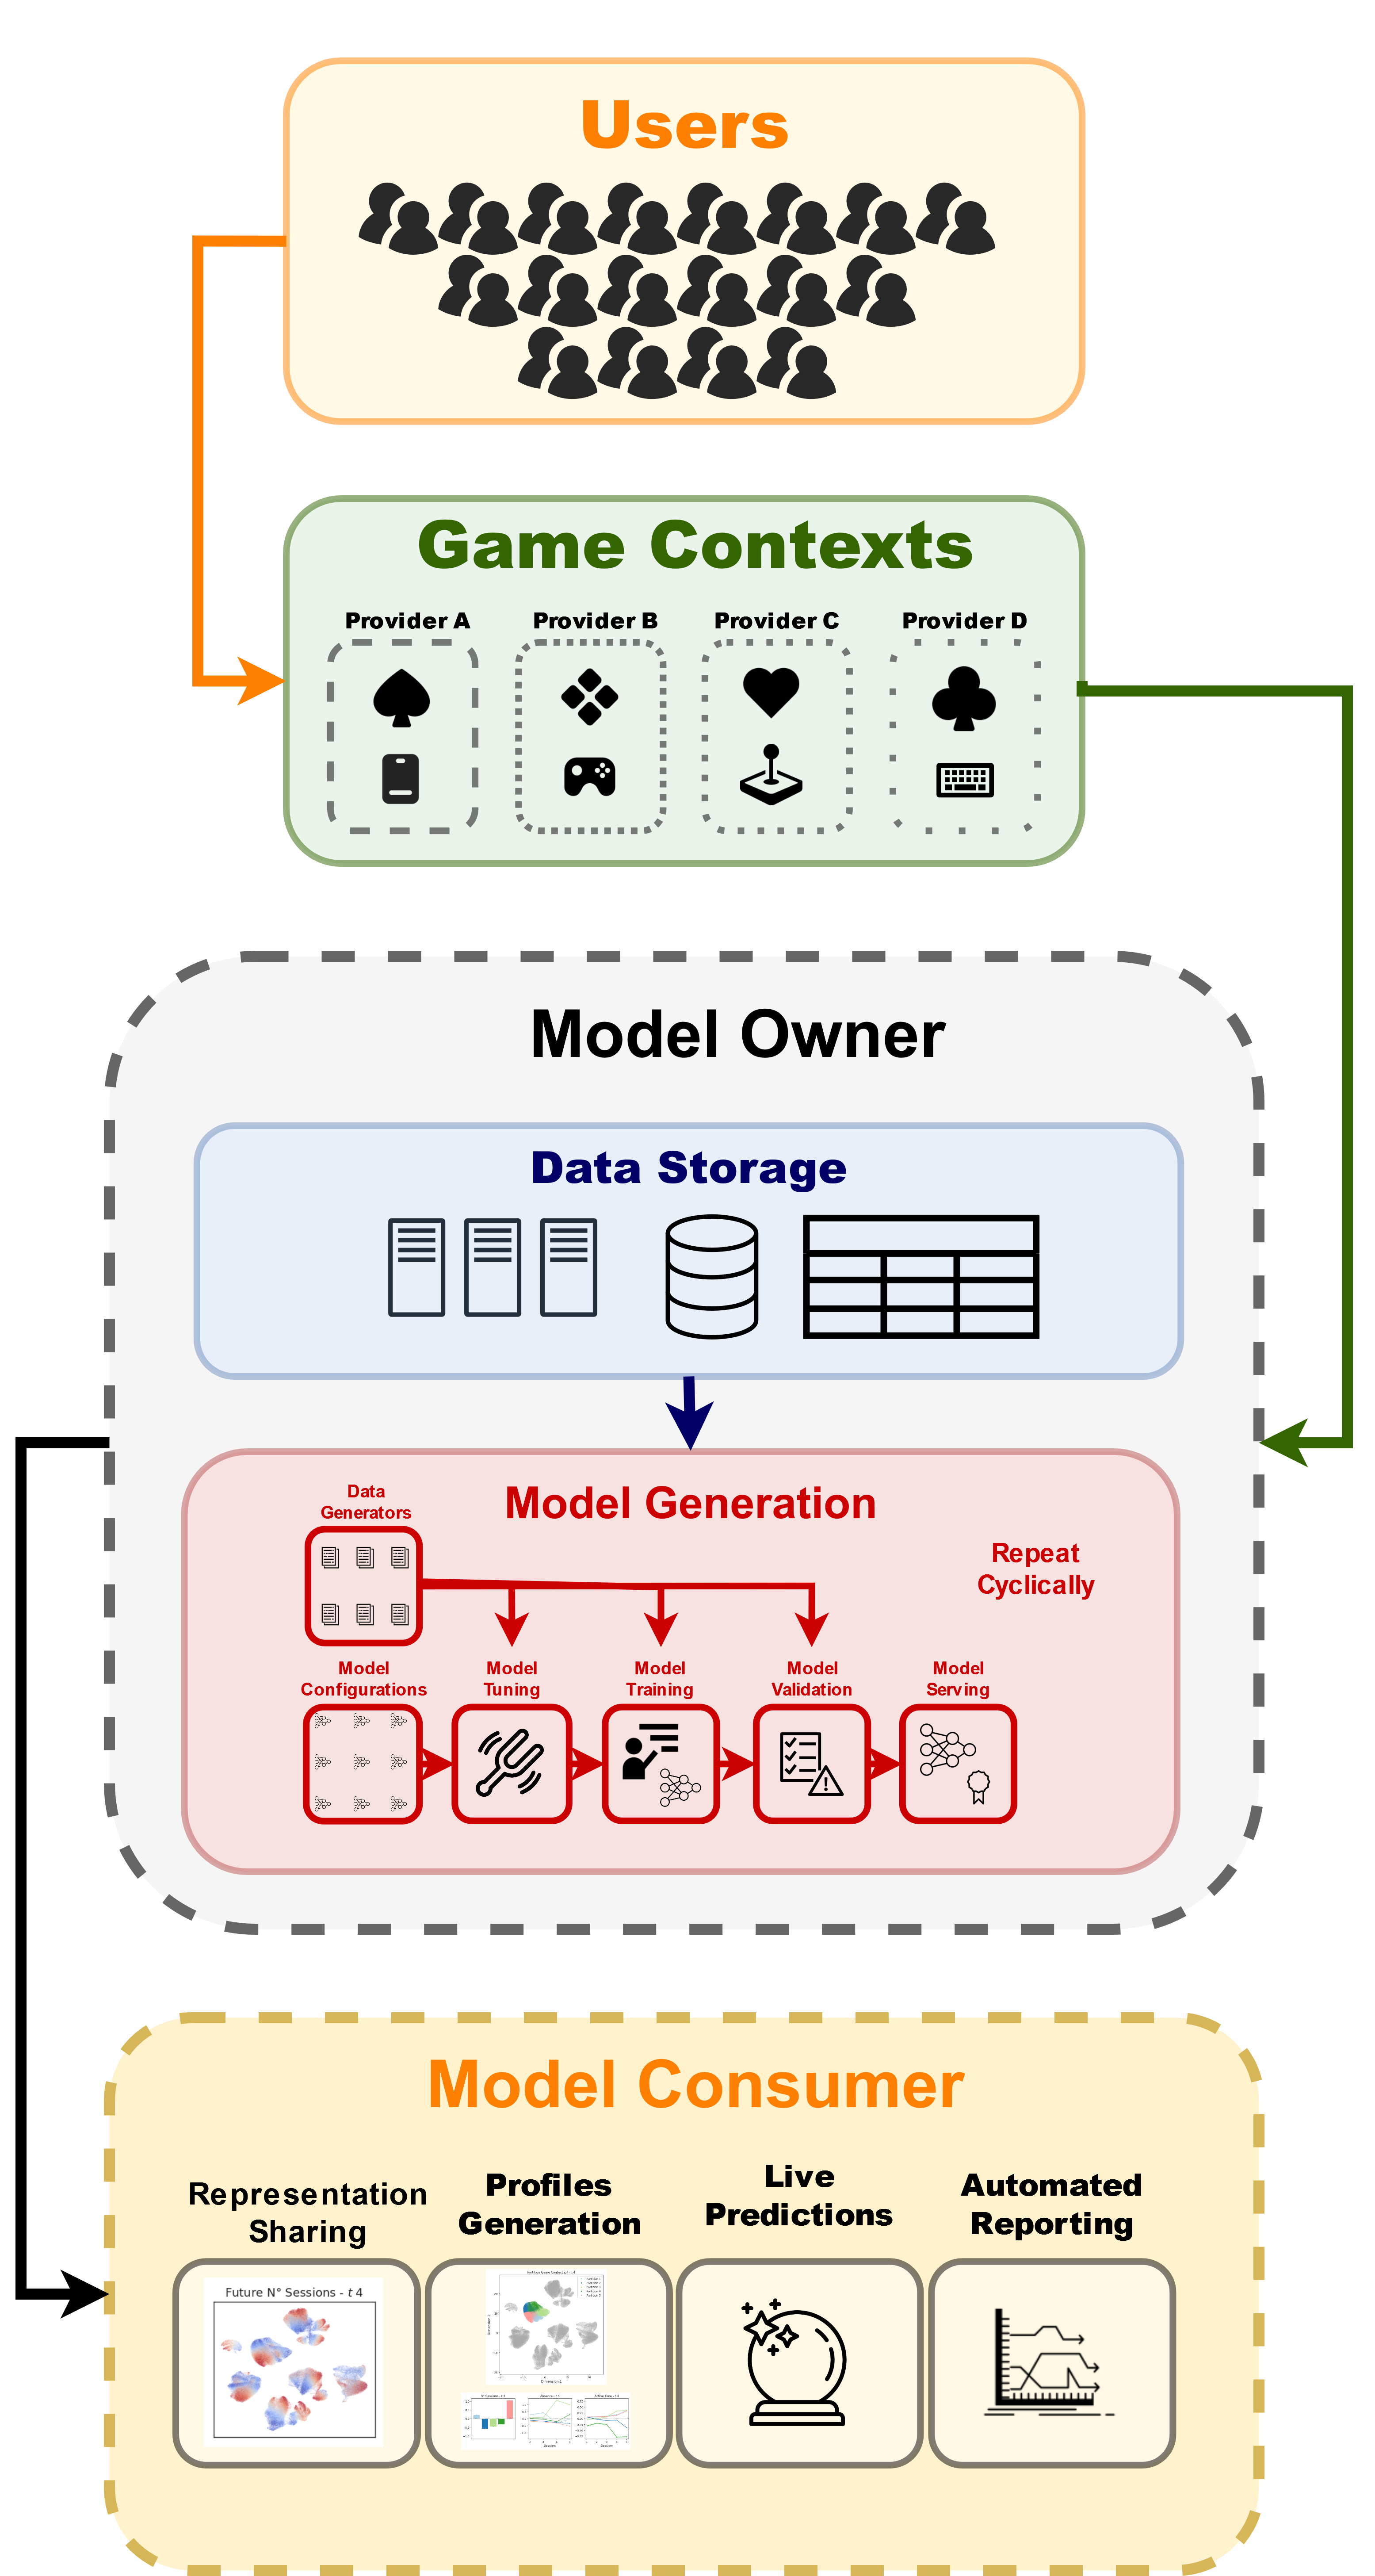
\includegraphics[width=0.7\textwidth]{images/chapter_5/pipeline_diagram.png}
\caption[\textbf{Model Deployment Pipeline}]{The figure represents a simplified system diagram for a potential application of the improved RNN architecture. Solid lines represent low-level components in the system while dashed lines indicate high-level entities. Directional arrows represent the flow of operations inside the system.}
\label{pipeline}
\end{figure}

\subsection{Data Generation}
\label{data_generation}
This is the first component of the system and describes the entities generating the data that will then be used by the system. It is composed by two major elements: the users and the game contexts. 

The relationship between these two entities has already been described in chapter \ref{chapter_lit_review} and chapter \ref{chapter_theory_modelling} in particular. In line with the framework that we adopted through out this thesis we assume that each game context posses properties (defined by their structural characteristics) that might result more or less rewarding to different users. By means of repeated interactions with the game contexts the users learn about these properties and progressively updates latent representations of the various contexts. These representations, which as we said in chapters \ref{chapter_lit_review} and \ref{chapter_theory_modelling} are imbued with value, act by either promoting or demoting future engagement with the game contexts quantifiable by means of metrics of behavioural frequency and intensity.

The various game contexts can be managed by a single or multiple entities and are usually provided through different type of systems. For example, the game contexts utilized for this thesis were managed by a single entity (i.e., our partner company Square Enix Ltd.) and provided through an array of different hardware systems: smartphones, personal computers and gaming consoles. Ultimately, the software and console hardware make up the game context with which the users interact and within those lies the telemetry system in charge of recording the behavioural metrics and transmitting them to the relevant data storage systems.

\subsection{Model Owner}
\label{model_owner}
This component represents the entity responsible for the acquisition ad storage of data generated by the interactions between the users and the game contexts. It is also in charge of managing all the operations necessary for fitting a learning algorithm to the data and validating the derived model. 

It is relevant to highlight that the model owner usually corresponds one-to-one with the entity managing the game contexts but the two don't necessarily  have to coincide. In the context of federated learning  \cite{yang2019federated} for instance, a model owner might distribute copies of the learning algorithm across separate entities and only act as a pooling mechanism  once they have been fitted to the data \cite{kairouz2021advances}. In this case, the entities don't necessarily need to be known to the model owner or to each other, in fact this information must be kept hidden. Indeed, the aim of federated learning is to generate a global and robust model fitted on multi-source data while being compliant with strict privacy constrains \cite{yang2019federated, kairouz2021advances}. 

That said, for simplicity in this section we will focus on a situation where the model owner is one with the entity managing the game contexts.

\subsubsection{Data Storage}
Once the in-game behaviour resulting from the interaction between the users and the game contexts have been recorded by the telemetry system the information need to be transferred to a suitable storage system. Depending on the needs and technical capacity of the storage owner this can happen either via data streams or batch processing \cite{el2016game}. The component in charge of storing the data should also take care of conducting suitable Extract, Transform and Load (ETL) operations in order to move from the potential raw format in which the telemetries are collected to a more suitable one employable by the learning algorithm \cite{el2016game}. The ETL operations should also take care of all those sanity checks and pre-processing steps that are not directly relevant to the generation of the machine-learned model. This would correspond to the various filters and pre-processing steps that we mentioned in sections \ref{data_1}, \ref{data_2} and \ref{data_3}.

\subsubsection{Model Generation}
Once the raw information provided by the telemetry system has been processed, cleaned, organised and stored in a suitable tidy format a learning algorithm can be fitted to the data. In this case we assume the learning algorithm to be one of the three ANN architectures presented in chapter \ref{chapter_implementation_testing} and hence relying on the same operations presented in sections \ref{tuning_comparison_1}, \ref{tuning_comparison_2} and \ref{tuning_comparison_3} for tuning, fitting and validating.

\paragraph*{Data Generators} the first step in the model generation require the construction of appropriate mechanisms for feeding the data to the learning algorithm. Different generators will need to be created for the various steps of the process: one for tuning, one for training (i.e., fitting) and one for validating the generated model. It is worth noticing that the data generators do not only need to provide batches of the data to learning algorithm but are also in charge of applying the appropriated transformations (e.g., input scaling) in such a way that no information leaking is occurring and to adopt adequate randomisation strategies so to not introduce biases during the model fitting.

\paragraph*{Model Configurations} simultaneous to the construction of the data generators is the the creation of multiple architectural configurations. This step is motivated by the use of HyperBand \cite{li2017hyperband} for the search of the optimal hyperparameters. Indeed, as we specified in chapter \ref{chapter_implementation_testing} HyperBand works by iteratively training a large pool of models instantiated with a random selection of hyperparameters and progressively pruning those showing poor out-of-sample perfromance. At this stage the only thing that needs to be specified are the hyperparameters to optimize and the boundaries of the search space. Routinely validation checks should also be included in this stage for removing from the pool of potential configurations those that resulted to be corrupted. Indeed certain hyperparameters configurations might make training or even model instantiation infeasible.

\paragraph*{Model Tuning} once the model configurations have been generated it is possible to search for the best performing hyperparameters using the aforementioned HyperBand algorithm \cite{li2017hyperband}. It is worth noticing that at this stage not just the hyperparameters relative to the architecture can be optimized but also those associated with other relevant components such as the optimizer (e.g., the optimizer learning rate). The amount of data assigned to the data generator used at this stage should strike a balance between efficacy and waste. If too little data are used, the hyperparameters search might produce sub-optimal results. However going to the other extreme might hurt the training stage as the data used for searching the best model configuration cannot be re-used. What needs to be specified is the budget to be given to the tuning algorithm. Despite HyperBand being extremely parallelizable \cite{li2017hyperband} this a choice should still be informed by the available resources and time constrains.

\paragraph*{Model Training} a this stage the best model configuration should be fitted to the bulk of the available data. It is worth noticing that depending on the size of the training data this stage might be very resource intensive. However fitting should not necessarily always be carried out on the entire amount of data. For example, if the algorithm has recently been though a full training stage (e.g., leveraging all the available historical data) an update based on the latest available data might be sufficient. Moreover if strong resources constrains are present, it might be possible to fit the learning algorithm using a suitably defined random sample of the original data. This of course depends on the number of parameters in the model, the complexity of the learning task and the heterogeneity and size of the available data. Fitting model to the data should be carried out until convergence or a suitably defined level accuracy is achieved, again the choice of such level might be dictated by time or resources constrains. In this regard, convergence should always be assessed and monitored through out-of-sample metrics with the option of triggering an early stopping policy if improvements are not observed for a long period of time (see details specified in sections \ref{tuning_comparison_1}, \ref{tuning_comparison_2}, \ref{tuning_comparison_3}). What is important at this stage is to create checkpoints of the model state whenever out-of-sample accuracy reliably improves and to keep detailed logs of the fitting procedure. The first avoids to wasted efforts if the optimisation process suddenly diverge or come to an abrupt end (e.g., due to technical issues), the second allows to keep track of relevant metrics useful for assessing if and how convergence is reached.

\paragraph*{Model Validation} once the learning algorithm has been fitted on the data it is necessary to validate the model in order to verify its usability in a production environment. The validation process can be extremely articulated and in large part depends on the needs of the model owner, however two main aspects should certainly be validated. First, a series of tests should be conducted in order to verify that basic functionalities are not disrupted, in our case for example we might want to make sure that the model is able to produce predictions and representations, that these are within critical boundaries (e.g., no extremely large or small values are present) and show particular properties (e.g., statistical or distributional ones). Second, the convergence and accuracy of the model should be assessed and compared against a critical lower bound or the perfromance of a naive approach (e.g., we provided some examples of these in sections \ref{competing_models_1}, \ref{competing_models_2} and \ref{competing_models_3}). Convergence can be assessed running automated tests on the logs created during Model Training checking for example the difference between in-sample and out-of-sample perfromance, variations in the $l2$ norm of the error gradient or in the parameters values \footnote{We suggest to consult \cite{bengio2017deep} for a more exhaustive list of checks.}. Accuracy can be evaluated by assessing model perfromance on a test set and then comparing it against the aforementioned benchmarks. In this case statistical approaches based on inference can be used for evaluating if the expected gains provided by the model lie outside of a Region Of Practical Equivalence (ROPE) and can justify the cost associated to deploy the model in production (an example of this can be found in Appendix \ref{appendix_ancillary_perf}).

\paragraph*{Model Serving} once the model has been validated it is possible to deploy it within a production environment. The frequency at which the model is queried for obtaining predictions or representation depends on the needs of the model consumer and again the available resources. For example, a demanding streaming approach might be needed for supporting live predictions or a system aiming to react to a rapid turnover of large volumes of users. On the other hand, a conventional scheduled job executing a prediction pipeline on much more relaxed schedule (e.g., once a day or even once a week) might be more than sufficient for generating static KPI reports and profiles.

The model generation process should be repeated end-to-end on a regular basis depending on how much distributional drift is expected in the data. However, parts of it like Model Training, Validation and Serving might be executed independently on a much more frequent schedule. 

\subsection{Model Consumer}
The model consumer identifies the entity interacting with the model and leveraging its outputs. As specified in section \ref{model_owner} this doesn't necessarily have to correspond to the model owner but it is supposed to be identified in at least one of the entities managing the game contexts. Again, for simplicity we will assume that in this case they all corresponds to the same entity. The model consumer shouldn't have direct access to the algorithm generated by the model owner nor should be able to alter its inner working (e.g., it should be able to re-fit the algorithm on a new set of the data), its only focus should be to consume its output for different type of applications. We will now proceed at briefly illustrating some of these applications.

\subsubsection{Representation Sharing}
As we described in chapters \ref{chapter_theory_modelling} and \ref{chapter_repr_anal}, the latent representation inferred by the different types of RNN architectures can be thought as an approximation of the saliency that an individual might attribute to interacting with a specific game object (i.e., a game context). We can think of it as compressed trace of the state of a user (or a group of users) indicative of the amount of future engagement that we can expect from them. 

As we have seen in section \ref{representation_env_even_contr}, this representation can be constructed from different types of inputs, being them the intensity of historical interactions with the game context or the sequences of game mechanics with which the user interacted. 

In this view, the inferred representation can be seen as a set of features extracted by the ANN architectures (see sections \ref{artificial_neural_networks} and \ref{manifold_learning}) which can then be made available to other learning algorithms in order to improve their perfromance. For example, a recommender system might leverage the representation derived by the game events inputs in order to produced personalized suggestions for contents that are more likely to foster engagement \cite{bertens2018machine}. Similarly, systems aiming to compute lifetime value (LTV) indexes might benefit from a representation informative of the  amount of future gaming behaviour expected by a group of users. Indeed such systems rely on two major components for deriving the LTV index: the avergae expenditure from a group of users along their expected amount of future playing behaviour  \cite{chen2018customer}.

\subsubsection{Profiles Generation}
\lorem

\subsubsection{Live Predictions}
\lorem

\subsubsection{Automated Reporting}
\lorem

\section{Discussion}
In this chapter we presented the design of a system aimed at leveraging the modelling approach described in this thesis for automated engagement prediction and quantification. 

We first highlighted some ethical considerations that should be taken into account when developing and deploying such system, posing particular attention to the issue of fairness.

We then described why an industry player might be interested in such system and why it is important to rely predictive approaches for taking "proactive" actions towards the improvement of user engagement and retention.

Subsequently we proceeded at describing the various components  